\subsection{Feedback loops}

When there is a lack of feedback from customers/users, then someone has to decide.


when there are multiple competing objectives among different stakeholders in a zero sum use of resources, how to determine what's best? Typically there are feedback loops to guide progress. When feedback loops are weak or not present, then the most powerful stakeholder (which is distinct from the biggest or loudest) will dominate. 

\subsubsection{Special interest groups}

when there is a benefit to a small group and the cost is to a larger group

\subsubsection{Spending taxpayer dollars}

Suppose I earn \$100,000 and the tax rate is 30\%. Then my tax money sent to the government is \$30,000.

"In 2021, the [US] government collected \$4.05 trillion in revenue."
\footnote{source: Government Revenue | U.S. Treasury Data Lab}

My taxes of \$30,000 is
30000/4050000000000 = 0.00000074\%

When I do not maximize the effectiveness of \$1,000,000 of government money, of that misallocated money \$0.0074, or about one penny, was taxes I paid. The feedback loop is weak.

Federal pay is limited to about \$220,000\footnote{https://en.wikipedia.org/wiki/Executive\_Schedule}, so that raises the feedback to 2 pennies.

The lack of feedback allows waste to go unfelt. There's no immediate consequence.
Waste is indistinguishable from not enough funding or insufficient skills 




Feedback loop:
\begin{center}
\begin{figure}[ht]
    \centering
    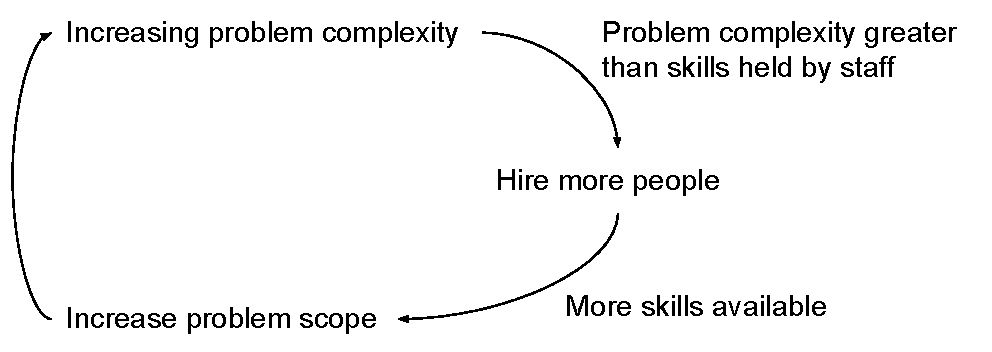
\includegraphics[width=0.8\textwidth]{images/feedback_loop_complexity_and_staffing}
    \caption{Complexity requires more staffing; having more staff means more skills are available; under-utilized staff skills make room for more scope; more scope adds to complexity.}
    \label{fig:complexity_and_staff_growth}
\end{figure}
\end{center}

\subsubsection{TSA agent making a fair decision}
% https://graphthinking.blogspot.com/2017/09/a-simple-illustration-of-bureaucracy.html
I was going through passport control. There was a TSA officer directing people into one of two lines. Both lines were long. The lines were not of equal length. Both lines terminate at a bunch of passport checking agents. Each passport check takes a minute. Passport checking TSA officers operate independently and concurrently.


The TSA officer's perspective is that there are two long lines. His procedure is two balance the two lines (for fairness). He does this by pointing people into one of the two lines, with his choice driven which line has room available.

Two people enter and are directed by the TSA officer. The first person is directed left, the second goes right. The TSA officer's job is completed.

The person in the left line finishes 5 minutes before the person in the line on the right. This difference in completion time is frustrating is frustrating for the person who is in the line on the right.

Because the lines are not of equal length, balancing the start of the line is an suboptimal method. The consequence is that what seems fair to the TSA officer ends up not being fair for people going through the line. The TSA officer had incomplete information -- the lines are not of equal length. Because the TSA officer isn't exposed to the consequence of is approach, he doesn't get feedback on whether it is suboptimal or not.

Lesson: if the people making decisions do not experience the consequences of those decisions, then they are not incentivized to improve decision making.

The person in the longer line feels frustrated. The negative feeling is due to a sense of powerlessness, and that the situation is recurring, and a better solution is available.

The optimal solution in this situation is to have a single line feeding the multiple TSA passport checkers. This eliminates the need for the decision maker.


\subsubsection{Parking garage}
% source: 
% https://graphthinking.blogspot.com/2019/07/altering-feedback-loops-to-change.html
Bob parks his car in a parking garage every day. The parking garage owner charges \$20 per day for people to park their car.

Bob recently found that one of the exit gates for the parking garage is broken. If Bob uses that gate to leave the parking garage, the gate does not function and Bob cannot exit. Then Bob has to call the parking gate operator to request an exception (which is granted) and Bob can then exit that gate, avoiding the \$20/day charge.

This action (go to broken gate, request exception, avoid charge) has been repeated for a long time (months). Bob's motive is to avoid the \$20 parking charge; the cost is a mere phone call and a minor delay. This cheating behavior harms the parking garage owner's income. However, the parking gate operator, serving as intermediary, insulates the parking garage owner from the interaction with the cheater. The cheating behavior is small enough that the parking garage owner may not notice.


\subsubsection{Meeting time compared to theft}
% https://graphthinking.blogspot.com/2021/02/organizations-value-things-more-than.html

Source: \cite{1995_Grove}.

In large organizations, there can be significant bureaucracy associated with even small purchases. A multi-step review process may be incurred for a \$2000 acquisition.

Another measurement of value is that if an employee were to steal even \$200 worth of materials, the organization would likely punish that employee.


Those metrics apply to tangible goods, but not to people's time. Consider a meeting of 10 people and each person's cost is \$200 per hour. A wasted meeting is not unusual and certainly would not incur bureaucratic review processes. The cost to the organization is fiscally the same -- \$2000. Similarly, consider an employee who is late and causes a loss of productivity. Merely depriving the organization of \$200 worth of time is not punished in the same way theft is.

In fact, organizations default to meetings (even recurring meetings) rather than not meet. And being late to a meeting is accepted. 

We can debate the differences between theft of materials and theft of time. The financial argument is clear. 
